% =====================================================================
%  sections/sec4.tex —— 4 由六维 A_1 理论得到的 AD 点（原文 pp.13–21）
% =====================================================================
\section{由六维 $A_1$ 理论得到的 AD 点}
\label{sec:a1}

我们从六维 $A_1$ 理论出发，把它紧致化在带非正则穿刺点的黎曼面上。虽然没有找到任何新理论，但看清我们这套构造的若干普遍特征是有益的，这些特征随后要推广到更高秩。此外，用目前这套构造，我们能够求出它们的三维镜像理论、中心荷 $a$ 与 $c$，以及它们的 $\SU(2)$ 线性箭图 UV 完备等等。

我们需要先弄清楚：什么样的奇点组合才能在红外给出 SCFT。四维 $\sN{=}2$ SCFT 带一个 $U(1)_R$ 对称性，它在六维构造中有一个几何含义：它就是黎曼面的旋转对称性，因此余切丛的坐标 $z$ 与 $x$ 都在这对称性下变换。在正则奇点的情形，黎曼面上的 $z$ 坐标在这对称性下平凡变换，于是可以在任意亏格的黎曼面上放任意多个正则奇点。在非正则奇点的情形（若极点阶 $r>2$），$z$ 坐标按非平凡方式变换，因此奇点必须放在旋转对称性的不动点上。众所周知，带有不动点的 $U(1)$ 等距只可能出现在黎曼球上，而在这种情形不动点只能放在南极或北极。所以，要构造 AD 理论，最多只能放两个奇点。

按我们的分类，$\SU(2)$ Hitchin 系统有两种非正则奇点。全纯 Higgs 场的形式（奇点放在 $\infty$）是
\begin{equation}
\Phi = \lambda z^{n-2}\begin{pmatrix} 1 & 0\\ 0 & -1\end{pmatrix}
+ A_{n-1}z^{n-3} + \cdots + \frac{A_1}{z} + \cdots,
\label{eq:4.1}\tag{4.1}
\end{equation}
我们称之为 type I 奇点。另一个解是
\begin{equation}
\Phi = \lambda z^{n-5/2}\begin{pmatrix} 1 & 0\\ 0 & -1\end{pmatrix}
+ A_{n-1}z^{n-7/2} + \cdots + \frac{A_2}{z^{1/2}} + \cdots
\label{eq:4.2}\tag{4.2}
\end{equation}
$z$ 平面上有一条割线；跨过割线时要做一次规范变换，才能使解自洽。注意这里没有一阶项，因此这个奇点不编码质量参数。我们称之为 type II 奇点。

下面我们论证只允许有一个非正则奇点；若已经有一个非正则奇点，则只能再打开一个正则奇点。证明如下。若把两个非正则奇点分别放在 $z=0$ 与 $\infty$，则谱曲线具有形式
\begin{equation}
x^2 = z^N + \cdots + \frac{\lambda^2}{z^M}.
\label{eq:4.3}\tag{4.3}
\end{equation}
这里 $M\ge 3$，$\lambda$ 是来自高阶极点的系数。我们还用标度变换把 $z^N$ 的系数取为 $1$。若这定义了一个 SCFT，则 $[\lambda^2]=\frac{2(N+M)}{N+2}>2$，意味着它是一个库仑分支算子；但这与「来自高阶极点系数的参数应当是维数小于一的耦合常数」这一事实矛盾。综上，能定义 AD 理论的奇点配置只有下面两种：
\begin{enumerate}
  \item 黎曼球上有一个非正则奇点。
  \item 球的南极有一个非正则奇点，北极有一个正则奇点。
\end{enumerate}

\subsection{AD 点的构造}
\label{sec:4.1}

\subsubsection{一个非正则奇点：$(A_1,A_{N-1})$ SCFT}
\label{sec:4.1.1}

四维理论由在黎曼球无穷远处放一个非正则奇点来定义。先说明如何从几何数据读出耦合常数、质量参数的个数与库仑分支的维数。

type I 奇点对 Hitchin 模空间的局部维数是 $2n$。$A_{n-1},\dots,A_2$ 中共有 $n-2$ 个参数，而 $A_1$ 中编码一个质量参数。$A_{n-1}$ 中的那个参数可以用平移不变性消去，因此有效只有 $n-3$ 个耦合常数。计入整体贡献后，Hitchin 模空间的维数是 $2n-6$；而 Hitchin 纤维化底空间的维数是 $n-3$，它等于库仑分支的维数，见表 \ref{tab:1}。

type II 奇点对 Hitchin 模空间的局部维数同样是 $2n$；我们仍然在 $A_{n-2},\dots,A_2$ 中有 $n-3$ 个参数（同样用平移不变性消去 $A_{n-1}$ 中的参数），但没有质量参数。Hitchin 纤维化的底空间维数也是 $n-3$，见表 \ref{tab:1}。

\begin{table}[tbp]
\centering
\caption{黎曼球上一个非正则奇点的几何数据。高阶极点中的一个参数用平移不变性消去了。}
\label{tab:1}
\begin{tabular}{lcccc}
\toprule
 & 极点阶 & 底空间维数 & 一阶极点 & 高阶极点\\
\midrule
Type I  & $n$        & $n-3$ & 1 & $n-3$\\
Type II & $n-1/2$    & $n-3$ & 0 & $n-3$\\
\bottomrule
\end{tabular}
\end{table}

Seiberg--Witten 曲线由计算 Hitchin 纤维化的谱曲线得到：
\begin{equation}
x^2 = \Tr(\Phi^2) = z^N + u_2 z^{N-2} + \cdots + u_N .
\label{eq:4.4}\tag{4.4}
\end{equation}
容易看出：type I 奇点对应 $N = 2n-4$，type II 奇点对应 $N = 2n-5$。这一类理论被称为 $(A_1,A_{N-1})$ 理论，这个名字来自一个事实：该理论的 BPS 箭图是 $A_1$ 与 $A_{N-1}$ 两个 Dynkin 图之积 \cite{3,17,31}。后文用一对李代数来标记理论时，总意味着 BPS 箭图具有两个 Dynkin 图之积的形状。

Seiberg--Witten 曲线可以很方便地从非正则奇点的牛顿多边形读出。牛顿多边形所界定的非负格点，代表 Seiberg--Witten 曲线中出现的单项式：坐标为 $(m,n)$ 的每个格点代表单项式 $x^mz^n$。带一个 $x$ 因子的单项式缺失，因为 $\Phi$ 无迹；而 $z = N-1$ 这条直线上的点则用平移不变性消去，见图 \ref{fig:3} 左图。

\begin{figure}[tbp]
\centering
% Figure 3 -- lattice pictures: left (A1,A5), right (A1,D7)
\begin{tikzpicture}[x=1pt,y=1pt,>=stealth,line width=0.5pt]
  \def\u{13.3}
  % ---------------- left panel ----------------
  \begin{scope}
    \draw (0,0) -- (0,106.7);          % vertical axis
    \draw (0,0) -- (120.4,0);          % horizontal axis
    \foreach \i in {1,2,3} {\draw ({\i*\u},0) -- ({\i*\u},{7.04*\u});}
    \foreach \j in {1,...,5} {\draw (0,{\j*\u}) -- ({4.05*\u},{\j*\u});}
    \foreach \j in {0,1,2,3,4,6} {\fill (0,{\j*\u}) circle[radius=1.8pt];}
    \fill ({2*\u},0) circle[radius=1.8pt];
    \draw (0,{6*\u}) -- ({2*\u},0);
  \end{scope}
  % ---------------- right panel ----------------
  \begin{scope}[xshift=159.7]
    \draw (0,{-4*\u}) -- (0,{8*\u});   % vertical axis
    \draw (0,0) -- (120.4,0);          % horizontal axis
    \foreach \i in {1,2,3} {\draw ({\i*\u},0) -- ({\i*\u},{7.04*\u});}
    \foreach \j in {1,...,6} {\draw (0,{\j*\u}) -- ({4.05*\u},{\j*\u});}
    \foreach \j in {-2,-1,0,1,2,3,4,5,6} {\fill (0,{\j*\u}) circle[radius=1.8pt];}
    \fill ({2*\u},0) circle[radius=1.8pt];
    \draw (0,{6*\u}) -- ({2*\u},0);
  \end{scope}
\end{tikzpicture}

\caption{左：$(A_1,A_5)$ 理论的图形表示，用标度不变性把 $z^6$ 项的系数定为 $1$，用平移不变性消去 $z^5$ 项。右：$(A_1,D_7)$ 理论的图形表示，注意 $z^5$ 项被打开了，它充当耦合常数。}
\label{fig:3}
\end{figure}

Seiberg--Witten 微分是 $\lambda = x\,\dd z$，$x$ 与 $z$ 的标度维数为
\begin{equation}
[x] = \frac{N}{N+2},\qquad [z] = \frac{2}{N+2}.
\label{eq:4.5}\tag{4.5}
\end{equation}
由此可以对 Seiberg--Witten 曲线中各个算子算出标度维数：
\begin{equation}
D(u_i) = \frac{2i}{N+2}.
\label{eq:4.6}\tag{4.6}
\end{equation}
若 $N = 2n-5$，则 $u_2$ 到 $u_{n-2}$ 的标度维数小于一，而 $u_{n-1}$ 到 $u_{2n-5}$ 是相关算子，于是库仑分支维数为 $n-3$，耦合常数也是 $n-3$ 个。对每一个相关算子 $u_i$，谱中都存在一个耦合常数 $m_i$，使 $D(u_i)+D(m_i)=2$。

类似地，若 $N = 2n-4$，则 $u_2$ 到 $u_{n-2}$ 是耦合常数，$u_{n-1}$ 的维数为一、是质量参数；$u_n$ 到 $u_{2n-4}$ 是库仑分支参数，总数为 $n-3$ 个。这些数据汇总在表 \ref{tab:2} 中。

\begin{table}[tbp]
\centering
\caption{由 Seiberg--Witten 曲线数出的物理参数。}
\label{tab:2}
\begin{tabular}{lcccc}
\toprule
 & 库仑分支 & 质量参数 & 耦合常数 & 奇点\\
\midrule
$(A_1,A_{2n-5})$ & $n-3$ & 1 & $n-3$ & Type I，阶 $n$\\
$(A,A_{2n-6})$   & $n-3$ & 0 & $n-3$ & Type I，阶 $n-1/2$\\
\bottomrule
\end{tabular}
\end{table}

\typo{表 2 第二行第一列原文印作 $(A,A_{2n-6})$，漏了下标 $1$，按第一行与上下文的写法应为 $(A_1,A_{2n-6})$。此外该行「奇点」一栏原文写的是 "Type I with order $n-1/2$"，但按表 1 与本节正文，极点阶为半整数的奇点是 type II（$N=2n-5$ 对应 type II，$N=2n-4$ 对应 type I）；该行的理论名 $(A_1,A_{2n-6})$ 与「质量参数为 0」都与 type II 自洽，可见是「Type I」写错了。两处均照录原文。}

比较表 \ref{tab:1} 与表 \ref{tab:2}，我们会发现：由 Seiberg--Witten 曲线数出的物理量个数，与几何数据的预言完全一致（已考虑平移不变性与标度不变性）。

事实上，$(A_1,A_2)$ 理论就是从带一个味的 $\SU(2)$ 得到的那个原初 AD 理论，而 $(A_1,A_3)$ 是从带两个味的 $\SU(2)$ 得到的 AD 理论。

\subsubsection{一个非正则奇点加一个正则奇点：$(A_1,D_{N+2})$ SCFT}
\label{sec:4.1.2}

我们可以在 $0$ 点再加一个正则奇点，以定义另一类 SCFT。几何上，这个正则奇点引入一个新的质量参数与一个 $\SU(2)$ 味对称性；此外库仑分支的维数增加一。Seiberg--Witten 曲线为
\begin{equation}
x^2 = \Tr(\Phi^2) = z^N + u_1 z^{N-1} + \cdots + u_N + \frac{u_{N+1}}{z} + \frac{m^2}{z^2}.
\label{eq:4.7}\tag{4.7}
\end{equation}
这一次，两个穿刺点把平移不变性固定住了，$u_1$ 无法消去，于是我们得到一个新的耦合常数 $u_1$，它与相关算子 $u_{N+1}$ 配对。$m^2$ 的维数为二，代表来自正则奇点的质量项。这一类理论被称为 $(A_1,D_{N+2})$ 理论，因为它的 BPS 箭图具有相应的形状。事实上，$N=-1$ 时什么都没有（没有基本表示）；$N=0$ 时它代表 $\SU(2)$ 的一个基本表示，见 \cite{3,32}。第一个非平凡的理论是 $(A_1,D_3)$ 理论，它同时也是从带两个味的 $\SU(2)$ 找到的 AD 点——这很自然，因为 $D_3$ 与 $A_3$ 的 Dynkin 图相同。$(A_1,D_4)$ 理论则是通过调节带三个味的 $\SU(2)$ 规范理论的质量参数与库仑分支算子找到的 AD 理论。

上面两类理论的 BPS 谱与墙穿越行为已在 \cite{3,33,34,35} 中研究过；线算子、面算子等延展对象则在 \cite{36,37} 中研究过。

\subsection{三维镜像}
\label{sec:4.2}

在正则奇点的情形，可以把四维理论紧致化在一个圆上，再流向深红外，得到一个相互作用的 三维 $\sN{=}4$ SCFT $A$。这个理论既有库仑分支也有希格斯分支。存在一个镜像理论 $B$，使 $B$ 的希格斯分支等于 $A$ 的库仑分支，反之亦然。奇妙的是，镜像理论总有拉氏量描述 \cite{38}：一个星形箭图。

类似地，把四维 AD 理论紧致化在圆上并流向深红外，我们也应当得到一个三维 $\sN{=}4$ SCFT。事实上，镜像理论同样可以通过粘合各奇点的箭图组件得到 \cite{39,40}。规则如下：
\begin{enumerate}[label=\textup{\alph*.}]
  \item 对每个正则奇点，接上一条如图 \ref{fig:4}b 所示的箭图支链。
  \item 对 type I 非正则奇点，接上如图 \ref{fig:4}a 所示的箭图。
\end{enumerate}
我们把正则奇点的 $U(2)$ 节点喷开成两个 $U(1)$ 节点，如图 \ref{fig:4}c 所示；粘合则通过认同这些 $U(1)$ 节点来实现，如图 \ref{fig:4}c 所示。从镜像理论库仑分支上的对称性，可以看出原理论增强了的味对称性。例如，$(A_1,A_3)$ 理论有 $\SU(2)$ 味对称性，这一点从它的三维镜像就能看出。该理论的三维镜像有两个 $U(1)$ 规范群，其间有两个双基本表示；由于其中一个 $U(1)$ 解耦，最终的镜像理论是带两个味的 $U(1)$，也就是 $T(\SU(2))$ 理论，而众所周知它的库仑分支上的对称性是 $\SU(2)$。

\begin{figure}[tbp]
\centering
% Figure 4 -- (a) n-2 bifundamentals between two U(1)'s; (b) leg of the regular singularity;
%             (c) U(2) split into two U(1)'s; (d) the glued quiver
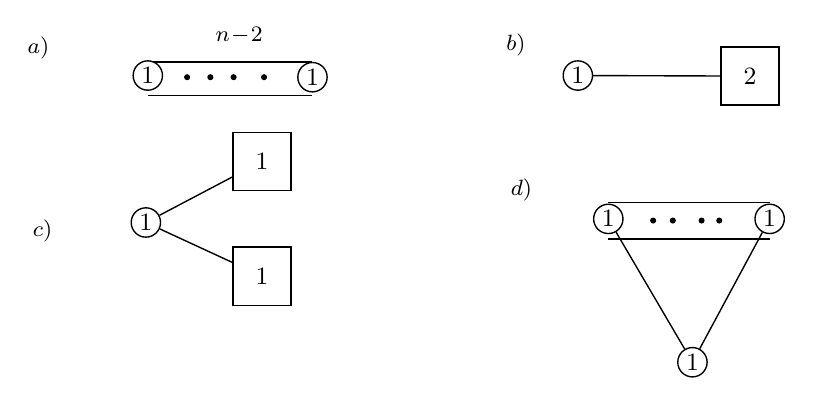
\begin{tikzpicture}[x=1pt,y=1pt,>=stealth,line width=0.5pt,
    nd/.style={circle,draw,fill=white,inner sep=0pt,minimum size=10.6pt,font=\small},
    sq/.style={rectangle,draw,fill=white,inner sep=0pt,minimum size=21pt,font=\small}]
  % ---------------- a) ----------------
  \draw (53,120.4) -- (112.5,120.4);
  \draw (53,108.35) -- (112.5,108.35);
  \node[nd] (a1) at (53,115.5) {1};
  \node[nd] (a2) at (112.5,114.9) {1};
  \foreach \x in {67.2,75.6,84.0,95.0} {\fill (\x,114.9) circle[radius=1.1pt];}
  \node[inner sep=0pt,font=\footnotesize] at (86,129.8) {$n\!-\!2$};
  \node[inner sep=0pt,font=\footnotesize] at (13.5,125.3) {$a)$};
  % ---------------- b) ----------------
  \node[nd] (b1) at (208.4,115.5) {1};
  \node[sq] (b2) at (270.6,115.3) {2};
  \draw (b1) -- (b2);
  \node[inner sep=0pt,font=\footnotesize] at (186,126.6) {$b)$};
  % ---------------- c) ----------------
  \node[nd] (c1) at (52.3,62.4) {1};
  \node[sq] (c2) at (94.3,43.0) {1};
  \node[sq] (c3) at (94.3,84.5) {1};
  \draw (c1) -- (c2);
  \draw (c1) -- (c3);
  \node[inner sep=0pt,font=\footnotesize] at (15,59.2) {$c)$};
  % ---------------- d) ----------------
  \draw (219.4,69.6) -- (277.7,69.6);
  \draw (219.4,56.5) -- (277.7,56.5);
  \node[nd] (d1) at (219.4,63.7) {1};
  \node[nd] (d2) at (277.7,63.7) {1};
  \node[nd] (d3) at (249.8,11.9) {1};
  \draw (d1) -- (d3);
  \draw (d2) -- (d3);
  \foreach \x in {235.6,242.7,253.1,259.5} {\fill (\x,63.1) circle[radius=1.1pt];}
  \node[inner sep=0pt,font=\footnotesize] at (188,74.1) {$d)$};
\end{tikzpicture}

\caption{(a)：极点阶为 $n$ 的 type I 非正则奇点对应的箭图，两个 $U(1)$ 群之间有 $n-2$ 个双基本表示，这就是 $(A_1,A_{N-1})$ 理论的三维镜像，其中 $N=2n-4$；(b)：正则奇点对应的箭图支链；(c)：把 (b) 的 $U(2)$ 味对称性喷开成两个 $U(1)$，以便把这条尾粘到 (a) 的箭图上；(d)：把 c 中的箭图尾与 a 中的箭图粘合，即 $(A_1,D_{N+2})$ 理论的三维镜像。}
\label{fig:4}
\end{figure}

\subsection{由线性箭图得到的 AD 点}
\label{sec:4.3}

在原始文献 \cite{6,11} 中，AD 点是通过调节 $\sN{=}2$ $\SU(2)$ SQCD 库仑分支上的参数找到的。人们自然希望为上一节找到的所有 AD 理论都配上类似的 UV 理论。我们没有去对原理论取各种标度极限，而是借助 Hitchin 系统来看工程化这些理论所需的奇点结构。SQCD 的非正则奇点极点阶较低，而对应的 AD 理论极点阶较高，因此 AD 理论的非正则奇点可以由对应 SQCD 的低阶奇点相撞得到。不过，还是有必要为奇点的碰撞找一条规则。

各种 $\SU(2)$ SQCD 的六维构造已在 \cite{3,41} 中给出。把这些 SQCD 的非正则奇点与相应的 AD 理论作比较，很容易猜出普遍规则，见图 \ref{fig:5}。例如，带一个味的 $\SU(2)$ 有一个 $n=2$ 的 type I 奇点，还有一个同样是 $n=2$ 的 type II 奇点；而对应的 AD 理论只有一个 $n=4$ 的 type II 非正则奇点，它可以看作两个阶为 $2$ 的非正则奇点相撞的结果。关键在于：新非正则奇点所编码的参数个数，应当等于原来两个奇点参数个数之和。这里我们假定原来那些参数（质量、库仑分支参数）全都成为 AD 理论的参数（质量、耦合常数、库仑分支参数）。

分析图 \ref{fig:5} 中其他情形之后，我们得到如下规则。

若至少有三个奇点，只能做下面这种碰撞：
\begin{enumerate}[label=\textup{\alph*.}]
  \item 把一个非正则奇点与一个正则奇点相撞，非正则奇点的极点阶加一，类型不变。
\end{enumerate}
若只剩下两个非正则奇点，则可以：
\begin{enumerate}[label=\textup{\alph*.},start=2]
  \item 把两个极点阶分别为 $n$ 与 $m$ 的非正则奇点相撞，新的非正则奇点极点阶为 $n+m$。
\end{enumerate}

\begin{figure}[tbp]
\centering
% Figure 5 -- A) Hitchin system for SU(2) QCDs (filled dot: type II irregular,
%             circle: type I irregular, cross: regular; number = integer part of pole order)
%             B) singularity structure of the corresponding AD theory
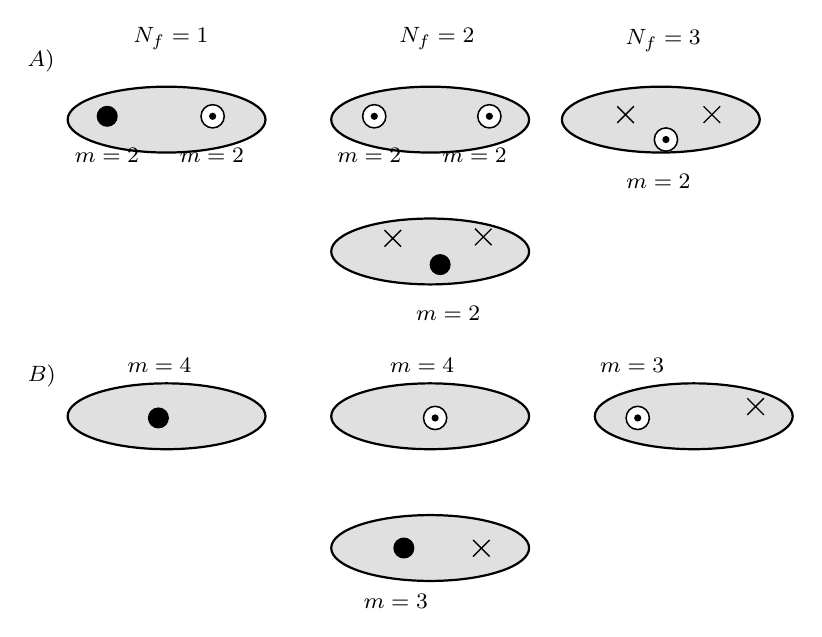
\begin{tikzpicture}[x=1pt,y=1pt,>=stealth,line width=0.5pt,
    ell/.style={draw,fill=black!12,line width=0.8pt}]
  % ================= A) =================
  \node[inner sep=0pt,font=\footnotesize] at (6.9,200.6) {$A)$};
  % N_f = 1
  \draw[ell] (52.25,179.4) ellipse[x radius=35.75pt,y radius=11.9pt];
  \fill (30.8,180.6) circle[radius=3.8pt];
  \draw[line width=0.55pt,fill=white] (68.9,180.6) circle[radius=4.2pt];
  \fill (68.9,180.6) circle[radius=1.3pt];
  \node[inner sep=0pt,font=\footnotesize] at (53.8,208.6) {$N_f=1$};
  \node[inner sep=0pt,font=\footnotesize] at (30.7,166.4) {$m=2$};
  \node[inner sep=0pt,font=\footnotesize] at (68.6,166.4) {$m=2$};
  % N_f = 2
  \draw[ell] (147.5,179.4) ellipse[x radius=35.75pt,y radius=11.9pt];
  \draw[line width=0.55pt,fill=white] (127.3,180.6) circle[radius=4.2pt];
  \fill (127.3,180.6) circle[radius=1.3pt];
  \draw[line width=0.55pt,fill=white] (168.9,180.6) circle[radius=4.2pt];
  \fill (168.9,180.6) circle[radius=1.3pt];
  \node[inner sep=0pt,font=\footnotesize] at (149.9,208.6) {$N_f=2$};
  \node[inner sep=0pt,font=\footnotesize] at (125.5,166.4) {$m=2$};
  \node[inner sep=0pt,font=\footnotesize] at (163.6,166.4) {$m=2$};
  % N_f = 3
  \draw[ell] (230.85,179.4) ellipse[x radius=35.75pt,y radius=11.9pt];
  \draw (215.1,178.2) -- (221.1,184.2);
  \draw (215.1,184.2) -- (221.1,178.2);
  \draw (246.3,178.2) -- (252.3,184.2);
  \draw (246.3,184.2) -- (252.3,178.2);
  \draw[line width=0.55pt,fill=white] (232.7,172.2) circle[radius=4.2pt];
  \fill (232.7,172.2) circle[radius=1.3pt];
  \node[inner sep=0pt,font=\footnotesize] at (231.7,208.0) {$N_f=3$};
  \node[inner sep=0pt,font=\footnotesize] at (230.0,157.0) {$m=2$};
  % second row of A)
  \draw[ell] (147.5,131.75) ellipse[x radius=35.75pt,y radius=11.9pt];
  \draw (131.0,133.5) -- (137.0,139.5);
  \draw (131.0,139.5) -- (137.0,133.5);
  \draw (163.7,134.0) -- (169.7,140.0);
  \draw (163.7,140.0) -- (169.7,134.0);
  \fill (151.1,127.0) circle[radius=3.8pt];
  \node[inner sep=0pt,font=\footnotesize] at (154.0,109.5) {$m=2$};
  % ================= B) =================
  \node[inner sep=0pt,font=\footnotesize] at (7.2,86.7) {$B)$};
  % m = 4 (type II)
  \draw[ell] (52.25,72.2) ellipse[x radius=35.75pt,y radius=11.9pt];
  \fill (49.3,71.6) circle[radius=3.8pt];
  \node[inner sep=0pt,font=\footnotesize] at (49.7,90.5) {$m=4$};
  % m = 4 (type I)
  \draw[ell] (147.5,72.2) ellipse[x radius=35.75pt,y radius=11.9pt];
  \draw[line width=0.55pt,fill=white] (149.3,71.6) circle[radius=4.2pt];
  \fill (149.3,71.6) circle[radius=1.3pt];
  \node[inner sep=0pt,font=\footnotesize] at (144.6,90.5) {$m=4$};
  % m = 3 (type I + regular)
  \draw[ell] (242.75,72.2) ellipse[x radius=35.75pt,y radius=11.9pt];
  \draw[line width=0.55pt,fill=white] (222.5,71.6) circle[radius=4.2pt];
  \fill (222.5,71.6) circle[radius=1.3pt];
  \draw (262.1,72.7) -- (268.1,78.7);
  \draw (262.1,78.7) -- (268.1,72.7);
  \node[inner sep=0pt,font=\footnotesize] at (220.5,90.5) {$m=3$};
  % second row of B)
  \draw[ell] (147.5,24.6) ellipse[x radius=35.75pt,y radius=11.9pt];
  \fill (138,24.6) circle[radius=3.8pt];
  \draw (163.0,21.5) -- (169.0,27.5);
  \draw (163.0,27.5) -- (169.0,21.5);
  \node[inner sep=0pt,font=\footnotesize] at (135.1,5.2) {$m=3$};
\end{tikzpicture}

\caption{A)：各种 $\SU(2)$ QCD 的 Hitchin 系统，黑点代表 type II 非正则奇点，圆圈代表 type I 非正则奇点，叉号代表正则奇点，数字是极点阶的整数部分。B)：由上述 QCD 找到的相应 AD 理论的奇点结构。}
\label{fig:5}
\end{figure}

利用上面的规则，不难为前面构造的 AD 理论找出 UV 理论。库仑分支为 $(n-1)$ 维的 AD 理论共有四个：$(A_1,A_{2n-1})$、$(A_1,A_{2n-2})$、$(A_1,D_{2n})$、$(A_1,D_{2n-1})$。按上述规则，可以定出其中一类理论的 UV 理论。其 UV 理论是 $\SU(2)-\SU(2)$ 线性箭图，两端挂不同数目的基本表示：
\begin{align}
\text{1. } &(A_1,A_{2n-2}) \to 0 - \underbrace{\SU(2)-\cdots-\SU(2)}_{n-1} - 1 ,\notag\\
\text{2. } &(A_1,A_{2n-1}) \to 1 - \underbrace{\SU(2)-\cdots-\SU(2)}_{n-1} - 1 ,\notag\\
\text{3. } &(A_1,D_{2n-1}) \to 0 - \underbrace{\SU(2)-\cdots-\SU(2)}_{n-1} - 2 ,\notag\\
\text{4. } &(A_1,D_{2n})   \to 1 - \underbrace{\SU(2)-\cdots-\SU(2)}_{n-1} - 2 .
\end{align}

下面解释第 1 种情形的碰撞规则，其他理论可类似理解。该线性箭图理论有一个阶为 $2$ 的 type I 奇点、一个阶为 $2-1/2$ 的 type II 奇点，以及 $n-2$ 个正则奇点。先把 type I 奇点与那些正则奇点相撞，得到一个阶为 $n$ 的 type I 奇点；最后再与 type II 奇点相撞，得到一个更高阶（$n+3/2$）的 type II 奇点，它正是 $(A_1,A_{2n-2})$ 理论所需的那个。UV 理论总共有 $2n-2$ 个参数，红外理论同样有 $2n-2$ 个参数。

\subsection{中心荷 $a$ 与 $c$}
\label{sec:4.4}

计算本节构造的 AD 理论的中心荷 $a$ 与 $c$，有两条路。第一条是使用下面两个公式
\begin{equation}
(2a-c) = \frac{1}{4}\sum_{i=1}^{r}\bigl(2D(u_i)-1\bigr),\qquad
a-c = \frac{1}{24}(n_v - n_h).
\label{eq:4.8}\tag{4.8}
\end{equation}
第二个公式对弱耦合的自由理论成立；我们假定把 $n_v$ 与 $n_h$ 视为矢量多重态与超多重态的有效个数之后，它对强耦合理论同样成立。注意 $n_v-n_h$ 恰好是 SCFT 的「Higgs」分支维数的相反数。这个数等于镜像理论库仑分支的维数，而镜像有拉氏量描述，故容易计算。对 $N=2n$ 的 $(A_1,A_{N-1})$ 理论，三维镜像的库仑分支维数为一。

先把上面两个公式用到 $(A_1,A_{N-1})$ 理论，得到
\begin{equation}
2a-c = \frac{1}{4}\sum_{i=n+2}^{2n}\Bigl(\frac{4i}{2n+2}-1\Bigr)
= \frac{1}{4}\frac{(-1+n)(1+2n)}{(1+n)},\qquad
a-c = -\frac{1}{24}.
\label{eq:4.9}\tag{4.9}
\end{equation}
解上面的方程组，得到
\begin{equation}
a = \frac{-5-5n+12n^2}{24(1+n)},\qquad
c = \frac{3n^2-n-1}{6(n+1)}.
\label{eq:4.10}\tag{4.10}
\end{equation}
对 $N=2n$ 的 $(A_1,D_{N+2})$ 理论，利用「三维镜像的库仑分支维数为二」这一事实，可以做类似的计算：
\begin{equation}
2a-c = \frac{1}{4}\sum_{i=n+2}^{2n+1}\Bigl(\frac{4i}{2n+2}-1\Bigr) = \frac{n}{2},\qquad
a-c = -\frac{1}{12}.
\label{eq:4.11}\tag{4.11}
\end{equation}
解之即得中心荷
\begin{equation}
a = \frac{n}{2} + \frac{1}{12},\qquad c = \frac{n}{2} + \frac{1}{6}.
\label{eq:4.12}\tag{4.12}
\end{equation}

要计算 $N = 2n-1$ 时的中心荷，我们使用下面这个由拓扑场论导出的公式 \cite{20}：
\begin{equation}
a = \frac{1}{4}R(A) + \frac{1}{6}R(B) + \frac{5}{24}r,\qquad
c = \frac{1}{3}R(B) + \frac{1}{6}r,
\label{eq:4.13}\tag{4.13}
\end{equation}
其中 $r$ 是库仑分支的维数，而 AD 理论的 $h$ 为零；又
\begin{equation}
R(A) = \sum_{i}\bigl(D(u_i)-1\bigr),
\label{eq:4.14}\tag{4.14}
\end{equation}
这里的求和跑遍所有库仑分支算子，用显式的 Seiberg--Witten 曲线容易算出。$R(B)$ 与 Seiberg--Witten 曲线的判别式有关，一般极难计算。我们的想法是：假设 $R(B)$ 对每一类理论都是 $N$ 的普适函数，再利用 $N=2n$ 时的上述结果，定出 $R(B)$ 对 $N$ 的函数依赖关系。

\typo{原文 p.19 在式 (4.13) 前写「the following formula derived from topological field theory (3)」，其中引用的「(3)」编号有误；从上下文看，它指的是第 \ref{sec:general} 节的式 (2.8)。译文按 (2.8) 理解，并在此注出。后文 p.22 又两次以「formula (3)」指同一式。}

对 $N=2n$ 的 $(A_1,A_{N-1})$ SCFT，用 Seiberg--Witten 曲线给出的算子标度维数，得到（另见 \cite{42}）
\begin{equation}
N = 2n:\quad R(A) = \frac{n(n-1)}{2(n+1)}.
\label{eq:4.15}\tag{4.15}
\end{equation}
把已知的中心荷 $a$ 与 $c$ 代入上面那个公式，即得 $R(B)$ 的形式
\begin{equation}
(A_1,A_{N-1}):\quad R(B) = \frac{N(N-1)}{2(N+2)}.
\label{eq:4.16}\tag{4.16}
\end{equation}
类似地，对 $(A_1,D_N)$ 理论容易算出
\begin{equation}
N = 2n:\quad R(A) = \frac{n}{2},
\label{eq:4.17}\tag{4.17}
\end{equation}
并得到 $R(B)$ 的如下结果：
\begin{equation}
(A_1,D_{N+2}):\quad R(B) = \frac{N+1}{2}.
\label{eq:4.18}\tag{4.18}
\end{equation}
于是终于可以算出那些我们没有三维镜像构造的理论的中心荷，只需用 $R(B)$ 的显式形式。$N=2n-1$ 时 AD 理论的中心荷为
\begin{equation}
\begin{aligned}
(A_1,A_{N-1}):\quad & a = \frac{(n-1)(24n-5)}{24(2n+1)},\quad c = \frac{(n-1)(6n-1)}{6(2n+1)};\\
(A_1,D_{N+2}):\quad & a = \frac{n(8n+3)}{8(2n+1)},\quad c = \frac{n}{2}.
\end{aligned}
\label{eq:4.19}\tag{4.19}
\end{equation}
上述结果与 \cite{20,42} 完全一致。一个自洽性检验是：$(A_1,D_3)$ 与 $(A_1,A_3)$ 两个理论给出相同的答案，$a=\tfrac{11}{24}$、$c=\tfrac{1}{2}$。中心荷公式汇总在表 \ref{tab:3} 中。

\begin{table}[tbp]
\centering
\caption{由六维 $A_1$ $(2,0)$ 理论得到的 AD 理论的中心荷。}
\label{tab:3}
\begin{tabular}{llcc}
\toprule
 & 约束 & $a$ & $c$\\
\midrule
$(A_1,A_{N-1})$ & $N=2n$   & $\dfrac{-5-5n+12n^2}{24(1+n)}$ & $\dfrac{3n^2-n-1}{6(n+1)}$\\[6pt]
$(A_1,A_{N-1})$ & $N=2n-1$ & $\dfrac{(n-1)(24n-5)}{24(2n+1)}$ & $\dfrac{(n-1)(6n-1)}{6(2n+1)}$\\[6pt]
$(A_1,D_{N+2})$ & $N=2n$   & $\dfrac{n}{2}+\dfrac{1}{12}$ & $\dfrac{n}{2}+\dfrac{1}{6}$\\[6pt]
$(A_1,D_{N+2})$ & $N=2n-1$ & $\dfrac{n(8n+3)}{8(2n+1)}$ & $\dfrac{n}{2}$\\
\bottomrule
\end{tabular}
\end{table}

\subsection{更多奇点：与 $(A_1,D_{N+2})$ 理论耦合的规范理论}
\label{sec:4.5}

我们可以在任意黎曼面上放任意多个非正则奇点与正则奇点。这些理论是渐近自由理论；若把非阿贝尔味对称性规范化，这一点可以用 AD 理论对 $\beta$ 函数的贡献来确认 \cite{22}。物理上，物质部分是带正则穿刺点的三孔球（代表三基本表示），以及带一个非正则奇点与一个正则奇点的球（代表 AD 理论）。整个理论由把正则奇点的对角 $\SU(2)$ 味对称性规范化得到，例子见图 \ref{fig:6}。

在球上只有一个 type I 非正则奇点、外加若干正则奇点的情形，可以用前面讲的那套处方求出它的三维镜像，一个例子见图 \ref{fig:7}。这些理论被称为完备理论，其 BPS 谱已在 \cite{31} 中研究过；特别是，这些理论的 BPS 箭图属于有限变异型 \cite{43}。

\begin{figure}[tbp]
\centering
% Figure 6 -- (a) Riemann sphere with one irregular and two regular punctures,
%             (b) its degeneration limit: two fundamentals and an AD point
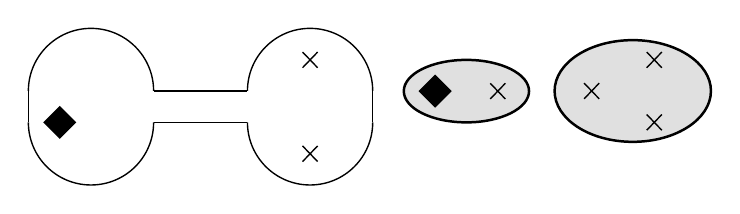
\begin{tikzpicture}[x=1pt,y=1pt,scale=1.05,transform shape,>=stealth,line width=0.5pt,
    bulb/.style={line width=0.5pt}, grey/.style={draw,fill=black!12,line width=0.9pt}]
  \def\cross#1#2{\draw (#1-2.6,#2-2.7) -- (#1+2.6,#2+2.7);\draw (#1-2.6,#2+2.7) -- (#1+2.6,#2-2.7);}
  % ---------- (a) dumbbell ----------
  \draw (51.6,35.0) arc[start angle=180,end angle=0,radius=21.55];
  \draw (51.6,24.2) arc[start angle=180,end angle=360,radius=21.55];
  \draw (51.6,24.2) -- (51.6,35.0);
  \draw (94.7,24.2) -- (127.0,24.2);
  \draw (94.7,35.0) -- (127.0,35.0);
  \draw (127.0,35.0) arc[start angle=180,end angle=0,radius=21.55];
  \draw (127.0,24.2) arc[start angle=180,end angle=360,radius=21.55];
  \draw (170.1,24.2) -- (170.1,35.0);
  % irregular puncture (filled diamond)
  \fill (56.7,24.2) -- (62.4,29.9) -- (68.1,24.2) -- (62.4,18.5) -- cycle;
  % two regular punctures
  \cross{148.55}{13.4}
  \cross{148.55}{45.7}
  % ---------- (b) the two pieces ----------
  \draw[grey] (202.35,34.95) ellipse[x radius=21.55pt,y radius=10.75pt];
  \fill (185.9,34.95) -- (191.6,40.65) -- (197.3,34.95) -- (191.6,29.25) -- cycle;
  \cross{213.15}{34.95}
  \draw[grey] (259.6,35.0) ellipse[x radius=26.9pt,y radius=17.5pt];
  \cross{245.45}{35.0}
  \cross{267}{24.2}
  \cross{267}{45.7}
\end{tikzpicture}

\caption{(a) 带一个非正则穿刺点与两个正则穿刺点的黎曼球。(b) 在它的「退化极限」下，物质是两个基本表示加上我们前面定义的一个 AD 点。}
\label{fig:6}
\end{figure}

\begin{figure}[tbp]
\centering
% Figure 7 -- the three dimensional mirror of the gauge theory of figure 6
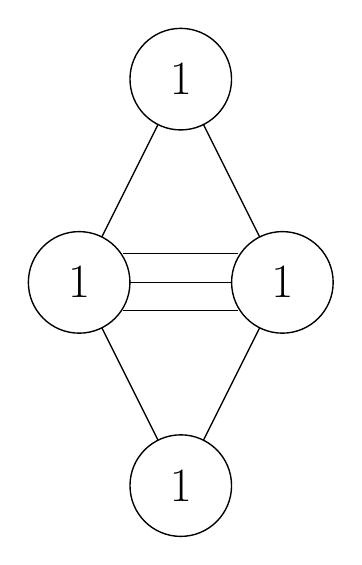
\begin{tikzpicture}[x=1.8pt,y=1.8pt,>=stealth,line width=0.5pt,
    nd/.style={circle,draw,fill=white,inner sep=0pt,minimum size=36.7pt,
               font=\fontsize{16.4}{19}\selectfont}]
  % the two horizontal links between the left and the right node
  \draw (24.4,47.7) -- (47.4,47.7);
  \draw (24.4,59.2) -- (47.4,59.2);
  % the four legs
  \draw (15.5,53.4) -- (35.9,94.2);
  \draw (35.9,94.2) -- (56.3,53.4);
  \draw (15.5,53.4) -- (35.9,12.6);
  \draw (35.9,12.6) -- (56.3,53.4);
  \draw (25.7,53.4) -- (46.1,53.4);
  % nodes
  \node[nd] at (15.5,53.4) {1};
  \node[nd] at (56.3,53.4) {1};
  \node[nd] at (35.9,94.2) {1};
  \node[nd] at (35.9,12.6) {1};
\end{tikzpicture}

\caption{上一图所述规范理论的三维镜像。}
\label{fig:7}
\end{figure}
